\documentclass[11pt]{article}

% --- PACKAGES ---
\usepackage[utf8]{inputenc}
\usepackage[T1]{fontenc}
\usepackage{lmodern}
\usepackage{mathptmx}
\usepackage[margin=1in]{geometry}
\usepackage{setspace}
\usepackage{titlesec}
\usepackage{authblk}
\usepackage{booktabs}
\usepackage{float}
\usepackage{graphicx}
\usepackage{upquote}
\usepackage{listings}
\usepackage{amsmath}
\usepackage{amssymb}
\usepackage[colorlinks=true, linkcolor=blue, citecolor=blue, urlcolor=blue]{hyperref}

\lstset{basicstyle=\ttfamily\small, columns=fullflexible, xleftmargin=4em,
        breaklines=true, keepspaces=true}

% --- STYLE ---
\onehalfspacing

\titleformat{\section}
  {\normalfont\Large\bfseries\scshape}{\thesection.}{1em}{}

% --- METADATA ---
\title{\textbf{Agentic Knowledge Graph Construction for Digital Twins:\\
A Multi-Agent LLM Pipeline for Industrial SOP Rule Extraction}}

\author{Dleflef}
\date{\today}

% ==============================================================================
\begin{document}

\maketitle

\begin{abstract}
Industrial Standard Operating Procedures (SOPs) encode safety-critical operational
rules across heterogeneous formats---narrative procedures, numeric threshold tables,
and role-zone permission matrices---that resist uniform extraction strategies.
Standard F1 metrics further conflate naming accuracy with content quality: in the
industrial Multi-Agent Knowledge extraction Synthetic dataset (iMAKS) benchmark,
many identifiers are annotated with conventions absent from the source text,
making exact-match metrics unreliable for evaluating operational correctness.

We adopt \emph{F1\textsubscript{content}}, a content-first metric that uses
Hungarian optimal assignment and SBERT similarity to evaluate operational correctness
independently of naming conventions.
A comprehensive single-agent grid search over five LLMs (4\,B to 20\,B parameters)
and ten prompting paradigms on the iMAKS corpus establishes a best single-agent
performance of F1\textsubscript{content}~=~0.728
(\texttt{gpt-oss-20b} with few-shot static prompting).

Building on these baselines, we design a multi-agent pipeline in which a
Document Type Coordinator routes each SOP to one of three specialised extractors.
The pipeline adds a Consensus Merger for deduplication, a Validator for
false-positive removal, an iterative Quality Gap Evaluator with re-extraction loops,
and an Identifier Canonicalizer.
An ablation study shows that the full pipeline achieves
F1\textsubscript{content}~=~0.823, surpassing the best single-agent baseline by
0.095 points (relative improvement of $\approx$13\%).
Removing the iterative judge loop drops F1\textsubscript{content} to 0.795;
removing the Validator decreases it to 0.776.
These results demonstrate that collaborative multi-stage refinement, rather than
dataset-specific prompt engineering, is the primary driver of extraction quality on
structurally heterogeneous industrial corpora.

The best extraction run is subsequently integrated into a Neo4j Knowledge Graph,
where the automatically extracted rules are overlaid on top of a hand-crafted
industrial ABox comprising 115 nodes and 341 edges representing the factory's
physical structure, sensors, anomaly events, maintenance procedures, and personnel
access rights.
A phase-2 graph coverage evaluation shows that the pipeline's extracted rules cover
14/14 anomaly events and 2/8 maintenance procedures, for an overall coverage of
72.7\% (above the 70\% design threshold), while a qualitative inspection of the
GOVERNS edges reveals systematic LLM failure modes in which temporal drift
thresholds are conflated with static alarm limits.
\end{abstract}

\tableofcontents
\newpage

% ==============================================================================
\section{Introduction}
\label{sec:intro}

\subsection{Context and Motivation}
In recent years, there has been a growing adoption of Digital Twins in complex
industrial domains. Within these environments, the Knowledge Graph (KG) is
increasingly recognised as the cognitive backbone of Digital Twins, though its
implementation is often hindered by the limitations of the current state of the
art. Industrial facilities generate knowledge across various simultaneous streams,
ranging from continuous numerical measurements produced by sensors to Standard
Operating Procedures (SOPs) that encode alarm thresholds and maintenance rules in
natural language.

Despite the potential of KGs to unify this data, there are significant bottlenecks
in high-quality KG construction, particularly concerning costs, scalability, and
semantic maintenance. Relying on manual extraction or centralised processing
pipelines is no longer viable for modern facilities. Consequently, there is a
pressing need for intelligent automation through multi-agent systems capable of
processing heterogeneous technical documentation and resolving inter-document
tensions.

\subsection{Literature Gaps}
A review of current KG construction methodologies reveals several critical gaps.
Primarily, there is an absence of systematic architectures for agent specialisation,
such as frameworks that clearly separate the roles of entity extraction, relation
validation, and ontology alignment agents. Furthermore, there are no comprehensive
comparative studies on how different agent collaboration strategies---whether
competitive, cooperative, or hierarchical---affect the quality of knowledge
extraction.

Additionally, there is limited work on incremental KG update mechanisms designed
to preserve semantic consistency over time. Finally, existing automatically
constructed KGs suffer from insufficient integration of temporal reasoning, which
is crucial for dynamic industrial environments where events are temporally
correlated.

\subsection{Objectives}
To address these limitations, this thesis outlines several primary objectives:
\begin{itemize}
    \item \textbf{Architecture Design:} Design a specialised multi-agent architecture
          for automated construction of KGs from heterogeneous technical documentation.
    \item \textbf{Conflict Resolution:} Implement robust conflict resolution mechanisms
          based on majority voting with configurable confidence thresholds.
    \item \textbf{Digital Twin Integration:} Map the extracted knowledge onto domain
          ontologies and integrate it seamlessly with a Digital Twin prototype.
    \item \textbf{Graph Implementation:} Build and populate a KG in Neo4j tailored for
          a specific industrial domain. This will be evaluated using the iMAKS
          (industrial Multi-Agent Knowledge extraction Synthetic) dataset, which
          simulates five days of operations at a food packaging facility.
    \item \textbf{System Evaluation:} Evaluate the proposed system using both
          quantitative and qualitative metrics, comparing its performance against
          traditional centralised NLP pipeline approaches.
\end{itemize}

% ==============================================================================
\section{Unstructured Data Parsing Strategy}
\label{sec:unstructured_parsing}

\subsection{Overview of Agent 1B}
Within the multi-agent architecture, the ingestion of unstructured documentation
is handled by Agent~1B. Industrial environments rely heavily on SOPs, which are
often distributed as unstructured or semi-structured PDF files. Converting these
documents into a format suitable for Large Language Models (LLMs) presents a
significant challenge: standard text extraction tools typically destroy layout
context---such as table structures and hierarchical headings---rendering the data
semantically incoherent for downstream extraction agents.

To address this, Agent~1B implements a robust, multi-stage extraction pipeline
consisting of vision-aware Markdown conversion, deterministic artifact sanitisation,
and context-aware chunking.

\subsection{Vision-Aware Markdown Extraction}
Traditional left-to-right PDF parsers fail when processing complex industrial
documents featuring multi-column layouts and dense data tables. To preserve spatial
and semantic context, Agent~1B utilises IBM's \texttt{docling} library, applying a
vision-language model approach to document conversion.

For PDF inputs, the agent processes the document visually to identify bounding boxes
around text, tables, and headers, exporting the reconstructed layout natively into
Markdown. For standard text files (\texttt{.txt}), the agent bypasses vision
extraction and reads the raw text directly. This Markdown representation ensures
that table boundaries and hierarchical sections are explicitly encoded as text
characters, which is critical for the subsequent entity and relation extraction
phases.

\subsection{Normalisation and Hallucination Scrubbing}
While vision-based extraction preserves layout, it introduces specific classes of
OCR artifacts and vision-model hallucinations. Agent~1B executes a strict
normalisation protocol (\texttt{\_normalise}) to sanitise the raw output before it
reaches the LLM context window.

\subsubsection{Ligature and Encoding Correction}
Industrial SOPs often contain specific mathematical or directional symbols that can
be corrupted by font encoding during PDF generation. Agent~1B explicitly corrects
known broken ligatures. For instance, the sequence ``fi'' is deterministically mapped
back to a right-arrow ($\rightarrow$), and ``fl'' is mapped to a down-arrow
($\downarrow$). Additionally, HTML entities are decoded, and escaped formatting
characters (e.g., \texttt{\\\_}) are sanitised to prevent Markdown injection errors
in downstream prompts.

\subsubsection{Table Cell Deduplication}
A common hallucination in layout-aware extraction models occurs when the model
generates overlapping bounding boxes over dense table cells, causing the underlying
text to be repeated sequentially (e.g., ``Inspect and lubricate HIGH Inspect and
lubricate HIGH'').

To resolve this without invoking an expensive secondary LLM call, Agent~1B deploys
a regex-based deduplication algorithm (\texttt{\_deduplicate\_table\_cells}). The
algorithm scans the document specifically for Markdown table rows (identified by
pipe \texttt{|} delimiters). Within each cell, it utilises a capture group to
identify any string of three or more characters that repeats itself sequentially,
collapsing the hallucination back into a single instance while repadding the cell
for clean Markdown formatting.

\subsection{Context-Aware Chunking Strategy}
LLMs possess finite context windows, and supplying an entire technical document
simultaneously degrades the performance of Named Entity Recognition tasks.
Conversely, splitting text arbitrarily mid-sentence destroys semantic meaning.

Agent~1B implements a context-aware chunking algorithm (\texttt{\_split\_into\_chunks})
that leverages the structural advantages of the extracted Markdown. The text is split
strictly at double newlines (\texttt{\textbackslash n\textbackslash n}), which
reliably represent paragraph or section breaks in Markdown.

The algorithm iterates through these natural paragraphs, merging them into an active
buffer until the buffer size exceeds a predefined maximum threshold of 2\,000
characters. To prevent the creation of uninformative microscopic chunks at the end
of a document, the algorithm enforces a minimum threshold of 200 characters; if the
final chunk falls below this limit, it is merged backward into the preceding chunk.
The fully sanitised and chunked text is then reassembled and saved as a uniform
\texttt{.txt} file, ready for the next step.

% ==============================================================================
\section{Evaluation Methodology}
\label{sec:evaluation}

Quantifying the quality of automatically extracted operational rules requires a
metric that is sensitive to semantic correctness while remaining robust to the
arbitrary nature of manually assigned identifiers. This section presents a
two-tier evaluation framework, implemented in \texttt{step3\_evaluation\_rules.py},
that measures extraction performance from complementary perspectives.

\subsection{Two Metrics: Strict Identifier Match and Content-First Similarity}
\label{sec:metrics}

\textbf{F1\textsubscript{strict}} (baseline): a conventional exact-match metric
based on rule identifiers. After normalising \texttt{ruleId} strings (lowercasing
and removing all non-alphanumeric characters), true positives are counted as the
intersection of ground-truth and predicted identifier multisets. Precision, recall,
and F1 are computed in the standard way. This metric provides a strict ceiling: in
the iMAKS dataset, many ground-truth identifiers are annotator conventions that
never appear verbatim in the source SOP texts; the maximum achievable
F1\textsubscript{strict} is therefore inherently limited.

\textbf{F1\textsubscript{content}} (primary): a content-first metric that ignores
identifiers entirely and instead evaluates how well the predicted rule content
matches the ground-truth rule content. It uses a class-weighted field-level
agreement score, aggregated via the Hungarian optimal assignment algorithm, and
then counts true positive matches above a threshold of $0.6$ to compute precision,
recall, and F1. This metric directly answers the question: \emph{Does the extracted
rule convey the same operational knowledge as the ground-truth rule?}

\subsection{Field Definitions and Class-Specific Weights}
\label{sec:field_weights}

The iMAKS rule schema contains twelve scored content fields, grouped into three
categories:
\begin{itemize}
\item \textbf{Text fields:} \texttt{condition}, \texttt{action}
\item \textbf{Numeric fields:} \texttt{critHi}, \texttt{warnHi}, \texttt{warnLo},
      \texttt{critLo}
\item \textbf{Categorical fields:} \texttt{class}, \texttt{station}, \texttt{sensor},
      \texttt{sensorType}, \texttt{severity}, \texttt{unit}
\end{itemize}
The field \texttt{ruleId} is not included in the content metric; its contribution
to operational knowledge is already captured by the numeric and categorical fields,
and it represents a naming convention rather than operational content.

Different rule classes place emphasis on different fields. For example, a
\texttt{ThresholdRule} hinges on its numeric boundaries, while an
\texttt{OperationalRule} relies primarily on its textual \texttt{condition} and
\texttt{action}. To capture this, the framework defines a static set of \emph{raw}
weights $w_f(c)$ for each field $f$ and class $c$, shown in
Table~\ref{tab:class_weights}. When computing content agreement, only the fields
that are non-empty in the ground-truth rule contribute; their weights are summed to
form the denominator, so weights are never pre-normalised. Fields absent from a
given class are omitted entirely from both numerator and denominator.

\begin{table}[htbp]
\centering
\small
\setlength{\tabcolsep}{3pt}
\caption{Field weights $w_f(c)$ by rule class. A dash (--) indicates the field is
         absent for that class and contributes nothing to the score.
         Weights are applied raw; the denominator is the sum over non-empty active
         fields in the ground-truth rule.}
\label{tab:class_weights}
\resizebox{\textwidth}{!}{%
\begin{tabular}{@{} l *{12}{c} @{}}
\toprule
\textbf{Class}
  & \texttt{class} & \texttt{station} & \texttt{sensor} & \texttt{sensorType}
  & \texttt{severity} & \texttt{unit}
  & \texttt{critHi} & \texttt{warnHi} & \texttt{warnLo} & \texttt{critLo}
  & \texttt{condition} & \texttt{action} \\
\midrule
\texttt{ThresholdRule}
  & 1.5 & 2.0 & 2.5 & 1.0 & 0.5 & 1.0 & 3.0 & 1.5 & 1.5 & 3.0 & 0.5 & 0.5 \\
\texttt{OperationalRule}
  & 1.5 & 2.0 & 1.5 & 0.5 & 1.0 & --  & 1.0 & --  & --  & 1.0 & 4.0 & 2.0 \\
\texttt{MaintenanceRule}
  & 1.5 & 2.0 & 2.5 & 1.0 & 1.5 & --  & --  & --  & --  & --  & 3.5 & 2.0 \\
\texttt{AccessRule}
  & 1.5 & 2.0 & --  & --  & 1.5 & --  & --  & --  & --  & --  & 2.0 & 1.5 \\
\bottomrule
\end{tabular}%
}
\end{table}

A fallback weight vector (class=1.0, station=1.5, sensor=1.5, severity=1.0,
condition=2.0, action=1.0) is used if a rule's class is missing or unrecognised.

\subsection{Field-Level Similarity Functions}
\label{sec:similarity_funcs}

Each field contributes a similarity score $s_f$ between a ground-truth value and
an extracted value:

\begin{itemize}
\item \textbf{Categorical fields} (exact match): $s_f = 1$ if the strings are
      identical after stripping and lowercasing, else $0$.
\item \textbf{Numeric fields} (relative tolerance):
      $s_f = \max(0,\; 1 - |a - b| / \max(|a|, |b|, \varepsilon))$,
      where $a$ is the ground-truth value and $b$ the extracted value. This yields
      1 when the numbers are equal and decays toward 0 as the relative difference
      increases.
\item \textbf{Text fields} (semantic similarity): $s_f$ is the cosine similarity
      between SBERT embeddings of the two text strings. The framework uses the
      \texttt{all-MiniLM-L6-v2} model from the Sentence-Transformers library, with
      embeddings cached to avoid redundant computation.
\end{itemize}

\subsection{Content Agreement Score}
\label{sec:content_agreement}

For a pair of ground-truth ($r_{\text{gt}}$) and extracted ($r_{\text{ext}}$) rules,
the content agreement $CA$ is defined as:

\begin{equation}
\label{eq:content_agreement}
CA(r_{\text{gt}}, r_{\text{ext}}) =
\frac{
  \displaystyle\sum_{f \in F_{\text{gt}}} w_f(c) \cdot s_f(r_{\text{gt}}, r_{\text{ext}})
}{
  \displaystyle\sum_{f \in F_{\text{gt}}} w_f(c)
}
\end{equation}

where $F_{\text{gt}}$ is the set of scored fields that are non-empty in the
ground-truth rule, $c$ is the ground-truth class, and $w_f(c)$ are taken from
Table~\ref{tab:class_weights} (or the fallback vector). This formulation ensures
that every ground-truth rule is evaluated solely on the information it actually
contains, and partial matches are rewarded proportionally.

\subsection{Hungarian Assignment and Content F1}
\label{sec:hungarian}

To compute F1\textsubscript{content}, the $n_{\text{gt}} \times n_{\text{pred}}$
matrix of content agreement scores is built, and the Hungarian algorithm (linear
sum assignment) finds the one-to-one pairing that maximises the total sum. A matched
pair is counted as a true positive if and only if its $CA$ exceeds a threshold of
$0.6$. Let $TP$ be the number of such qualifying pairs. Then:

$$P_{\text{content}} = \frac{TP}{n_{\text{pred}}}
\qquad \text{and} \qquad
R_{\text{content}} = \frac{TP}{n_{\text{gt}}}$$

$$F1_{\text{content}} = \frac{2\, P_{\text{content}}\, R_{\text{content}}}
                             {P_{\text{content}} + R_{\text{content}}}$$

This formulation directly rewards pairs that capture the essential operational
semantics while penalising spurious extractions; it is more robust than a soft sum
of scores because it avoids inflating precision when many low-quality rules are
produced.

\subsection{Implementation Details}
\label{sec:eval_impl}

\begin{itemize}
\item \textbf{SBERT caching:} The Sentence-Transformer model is loaded once as a
      singleton and embeddings are cached in a dictionary to avoid re-encoding
      repeated strings.
\item \textbf{Hardware acceleration:} The model automatically detects and utilises
      CUDA or MPS when available.
\item \textbf{Edge cases:} When either the ground truth or prediction list is empty,
      F1\textsubscript{content} is defined as 0.0.
\end{itemize}

% ==============================================================================
\section{Rule Extraction Grid Search Methodology}
\label{sec:grid_search}

Before introducing the collaborative multi-agent architecture, it is necessary to
establish a robust baseline for extracting operational rules from technical
documentation. To this end, a comprehensive grid search methodology was developed
to evaluate the performance of various LLMs and prompting paradigms on industrial
SOPs, using the F1\textsubscript{content} metric defined in
Section~\ref{sec:evaluation}.

\subsection{System Architecture and Experimental Parameters}
The grid search is orchestrated through a highly resilient, single-agent execution
pipeline. The system evaluates an array of models spanning parameter sizes from 4\,B
to 20\,B, specifically \texttt{ministral-3:14b}, \texttt{gemma3:12b},
\texttt{ministral-3:8b}, \texttt{qwen/qwen3-4b-2507}, and \texttt{gpt-oss-20b}.
To accommodate the dense technical nature of the documentation, the text input from
each SOP document is capped at 8\,000 characters.

The LLM connection parameters are configured to maximise stability during
long-running batch operations. The context window is explicitly set to 16\,384
tokens to ensure sufficient capacity for both the input text and the structured JSON
output. A strict timeout of 600 seconds (10 minutes) is enforced per API call, and
network resilience is handled via an exponential backoff mechanism that allows up to
three retries, starting with a 15-second base delay that doubles upon each failure.

For the majority of evaluated paradigms, the model temperature is set to $0$ and a
fixed random seed (default~42) is supplied to enforce deterministic, reproducible
outputs. The exception is the self-consistency paradigm, which utilises a
temperature of $0.3$ across three independent runs to generate a diverse set of
reasoning paths.

\subsection{Prompting Paradigms and Complexity Levels}
To systematically assess how LLMs interpret industrial logic, the grid search
categorises prompting strategies into four distinct complexity levels:

\begin{itemize}
    \item \textbf{Level~0 (Direct Extraction):} Includes the \texttt{naive} approach,
          which enforces a strict JSON schema without additional constraints.
          The \texttt{few\_shot\_static} paradigm enhances this by providing two
          concrete examples---one \texttt{OperationalRule} and one
          \texttt{ThresholdRule}---illustrating the required output format and numeric
          field mapping. Finally, the \texttt{graph\_informed} strategy introduces
          mandatory constraints, forcing the LLM to map its outputs to specific sensor
          naming conventions (e.g., \texttt{ST01\_FILLING\_TMP}).
    \item \textbf{Level~1 (Reasoning Before Action):} Introduces intermediate
          cognitive steps before JSON generation. The \texttt{cot\_basic} paradigm
          requires standard step-by-step reasoning, while \texttt{cot\_structured}
          enforces a strict five-step analytical process (mapping stations, identifying
          dependencies, extracting numeric bounds). The \texttt{pre\_act} paradigm
          requires the model to summarise the document's structure and rule categories
          before extraction.
    \item \textbf{Level~2 (Iterative Refinement and Ensemble Voting):} Incorporates
          multi-turn logic and ensemble strategies. The \texttt{self\_consistency}
          paradigm runs three independent extractions at temperature $0.3$ and then
          aggregates the results through a score-based voting mechanism
          (Section~\ref{sec:ensemble}). The \texttt{reflexion} strategy utilises a
          two-turn loop where the model critiques its own initial output for missing
          rules or imprecise numerics. The \texttt{reflexion\_guided} paradigm extends
          this to three turns, employing a rigid domain-specific checklist to verify
          completeness across stations, cross-station dependencies, and predictive
          maintenance protocols.
    \item \textbf{Level~3 (Tool Use / ReAct):} The \texttt{react\_abox} paradigm
          allows the model to actively verify sensor names against a localised
          Knowledge Graph (ABox). The LLM can halt its generation to emit a
          \texttt{VERIFY: <sensor\_name>} command. The system evaluates this request
          using fuzzy token-overlap matching and returns either a \texttt{SENSOR\_OK}
          confirmation or a \texttt{SENSOR\_NOT\_FOUND} warning with up to three
          syntactically similar suggestions.
\end{itemize}

\subsection{Ensemble Voting and Content Agreement}
\label{sec:ensemble}
The \texttt{self\_consistency} paradigm (Level~2) relies on an ensemble voting
mechanism to aggregate the results of three independent LLM calls. To determine
whether two independently generated rules describe the same operational constraint,
a \texttt{\_content\_agreement} algorithm calculates a weighted similarity score
(from 0.0 to 1.0).

Categorical fields (e.g., station, sensor) are evaluated using exact string
matching, while text fields (conditions and actions) are evaluated using a Jaccard
token-overlap approximation. Numeric fields within \texttt{ThresholdRule} instances
are subjected to a tolerance-based similarity calculation to prevent minor rounding
differences from invalidating a match.

The system implements a \texttt{score\_based} voting strategy by default. Rather
than requiring rules to share an identical \texttt{ruleId}, this strategy builds a
pairwise agreement matrix across all rules generated in the ensemble. If the
similarity score exceeds the predefined threshold of $0.55$, the rules are
clustered. A rule is only retained for the final output if it achieves a majority
consensus (appearing in at least 2 out of 3 runs).

\subsection{System Resilience and Output Parsing}
Given the tendency of LLMs to deviate from strict schemas, especially under high
token loads, the system includes extensive fallback mechanisms. Experiment state is
preserved via a JSON registry that marks runs as \texttt{partial} upon initiation
and \texttt{completed} only upon successful disk write, allowing interrupted grid
searches to resume seamlessly. Furthermore, a dedicated heartbeat thread
continuously logs timestamps to prevent silent hangs during prolonged API timeouts.

To extract valid data from malformed LLM responses, a cascading four-strategy JSON
parser is deployed. If standard parsing fails, the system attempts to repair
truncated JSON strings by balancing unclosed brackets. If the output contains
Markdown artifacts, regex extraction is used to isolate the data blocks. As a final
fallback, the parser iterates through the corrupted output to salvage any
individually well-formed rule objects.

% ==============================================================================
\section{Multi-Agent Extraction Pipeline Architecture}
\label{sec:pipeline}

Building on the grid-search findings, a staged extraction pipeline was designed
that combines specialised LLM agents under a graph-based orchestration framework.
The system treats rule extraction as a directed acyclic computation where each
stage contributes a specific quality-improving transformation. Implemented with
\texttt{LangGraph}, the pipeline dispatches LLM calls through local \texttt{Ollama}
or \texttt{LM Studio} endpoints, maintaining full data sovereignty with no cloud
dependency.

\subsection{System Constants and Operational Parameters}
\label{sec:constants}

Table~\ref{tab:constants} lists the tuned constants that govern the pipeline's
reliability. They balance recall, robustness on consumer-grade hardware, and output
fidelity by preventing JSON truncation.

\begin{table}[htbp]
\centering
\caption{Operational constants governing the pipeline.}
\label{tab:constants}
\begin{tabular}{@{} l p{4.0cm} p{7.5cm} @{}}
\toprule
\textbf{Constant} & \textbf{Value} & \textbf{Rationale} \\
\midrule
\texttt{SOP\_TEXT\_LIMIT}
  & 8\,000 characters
  & Covers the full text of each SOP while respecting model context windows. \\
\texttt{MAX\_OUTPUT\_TOKENS}
  & 16\,384
  & Provides sufficient room for the LLM to emit every extracted rule as a
    complete JSON array. \\
\texttt{LLM\_TIMEOUT\_SEC}
  & 600\,s
  & Accommodates large models on consumer hardware where inference can take
    several minutes. \\
\texttt{MAX\_RETRIES}
  & 3
  & Limits total attempts per LLM call before a node is considered failed. \\
\texttt{RETRY\_BASE\_DELAY}
  & 15.0\,s
  & Initial backoff delay; doubles on each subsequent retry. \\
\texttt{LLM\_NUM\_CTX}
  & 16\,384
  & KV-cache slots per request; must exceed prompt length to prevent silent
    truncation. \\
\texttt{MAX\_JUDGE\_RETRIES}
  & 1
  & Maximum re-extraction cycles triggered by the Quality Gap Evaluator. \\
\bottomrule
\end{tabular}
\end{table}

All LLM calls enforce a fixed random seed (\texttt{SEED~=~42}) and a temperature
of $0.0$ to ensure reproducibility.

\subsection{Shared State Management in LangGraph}
\label{sec:langgraph_state}

The computation graph operates on a typed dictionary, \texttt{PipelineState},
defined with \texttt{TypedDict}. Its key fields are:

\begin{itemize}
    \item \texttt{sop\_texts} --- mapping of source file names to their truncated
          SOP text (max 8\,000 characters).
    \item \texttt{doc\_types} --- mapping of source file names to document types
          (\textit{narrative}, \textit{tabular}, \textit{matrix}, \textit{mixed})
          as classified by the Coordinator.
    \item \texttt{extracted\_rules} --- an \texttt{Annotated} list with a sum
          reducer; outputs from parallel extractor nodes are automatically
          concatenated into a single candidate set.
    \item \texttt{merged\_rules} --- the consolidated rule set after merging and
          LLM adjudication.
    \item \texttt{validated\_rules} --- the rule set after the Validator's scrubbing
          and deterministic post-filtering.
    \item \texttt{normalized\_rules} --- final rule set with canonical identifiers
          assigned by the Normalizer.
    \item \texttt{retry\_files} --- dictionary of files flagged for re-extraction
          by the Judge, together with their document types.
    \item \texttt{retry\_count} --- number of judge-triggered retries performed in
          the current run (capped at \texttt{MAX\_JUDGE\_RETRIES}).
    \item \texttt{ablation} --- optional tag used to assemble simplified graph
          variants for ablation studies.
\end{itemize}

\subsection{Model Assignments and Node Configuration}
\label{sec:agent_config}

Each node in the graph is assigned a specific model and a dedicated system prompt.
The assignments, derived from grid-search evaluation on the iMAKS dataset, are
summarised in Table~\ref{tab:node_roles}.

\begin{table}[htbp]
\centering
\caption{Configuration of specialised nodes in the pipeline.}
\label{tab:node_roles}
\resizebox{\textwidth}{!}{%
\begin{tabular}{@{}llp{8cm}@{}}
\toprule
\textbf{Node} & \textbf{Model} & \textbf{Role} \\
\midrule
\texttt{Coordinator}
  & \texttt{qwen/qwen3-4b-2507}
  & Classifies each SOP as narrative, tabular, matrix, or mixed to select the
    appropriate extractor and judge checklist. \\
\texttt{Extractor~A} (narrative/mixed)
  & \texttt{gemma3:12b}
  & Extracts all rule classes (OperationalRule, ThresholdRule, MaintenanceRule,
    AccessRule) from prose-based documents. \\
\texttt{Extractor~B} (tabular)
  & \texttt{ministral-3:8b}
  & Extracts only ThresholdRule entries from sensor-threshold tables. \\
\texttt{Extractor~C} (matrix)
  & \texttt{gemma3:12b}
  & Extracts AccessRule entries from access-control and occupancy matrices. \\
\texttt{ConsensusMerger}
  & \texttt{ministral-3:14b}
  & Merges and deduplicates candidate rules, using deterministic heuristics first
    and escalating genuine conflicts to an LLM resolution. \\
\texttt{Validator}
  & \texttt{ministral-3:14b}
  & Pre-judge scrubber that removes false positives and recovers false negatives
    via a grounding check against the source text. \\
\texttt{QualityGapEvaluator}
  & \texttt{ministral-3:14b}
  & Iterative judge that detects class gaps, missing rules, quality issues, and
    conflicts; may trigger up to one re-extraction cycle. \\
\texttt{IdentifierCanonicalizer}
  & \texttt{qwen/qwen3-4b-2507}
  & Assigns canonical \texttt{ruleId} values while leaving all semantic fields
    unchanged. \\
\bottomrule
\end{tabular}%
}
\end{table}

\subsection{Stage Descriptions}
\label{sec:stages}

\subsubsection{Document Type Classifier}
\label{sec:classifier}

The \texttt{Coordinator} node reads the first 3\,000 characters of each SOP and
uses the \texttt{qwen/qwen3-4b-2507} model to produce a JSON object with the key
\texttt{doc\_type}. The classification rules are semantic: a document is
\texttt{tabular} if its dominant layout is a sensor threshold table with column
headers such as \texttt{CRIT\_LO}, \texttt{WARN\_LO}, etc.; \texttt{matrix} if it
presents an authorisation or occupancy grid; \texttt{mixed} if it interleaves prose
with structured maintenance tables or drift patterns; otherwise \texttt{narrative}.
This single determination later selects which specialised extractor and judge
checklist are used for that file.

\subsubsection{Specialised Extractors}
\label{sec:miners}

Three extractor nodes operate in parallel, each receiving only the documents that
match its document type.

\begin{itemize}
    \item \textbf{Extractor~A} (\texttt{gemma3:12b}) handles \texttt{narrative} and
          \texttt{mixed} SOPs. Its system prompt encompasses all four rule classes,
          multi-severity splitting (separate rules for WARNING and CRITICAL tiers of
          the same sensor), and the \emph{Physical Constraint Mapping} (PCM)
          principles. The prompt includes several few-shot examples and instructs the
          model to output a \texttt{"reasoning"} key alongside the \texttt{"rules"}
          list.
    \item \textbf{Extractor~B} (\texttt{ministral-3:8b}) handles \texttt{tabular}
          documents. The prompt restricts extraction to \texttt{ThresholdRule} entries,
          maps table columns to the four threshold fields, and enforces PCM so that no
          unit suffixes appear in numeric slots.
    \item \textbf{Extractor~C} (\texttt{gemma3:12b}) handles \texttt{matrix}
          documents. It extracts \texttt{AccessRule} entries for occupancy limits,
          acknowledgment deadlines, and any labelled access rules, again applying PCM
          to keep cell values verbatim.
\end{itemize}

Every extractor applies the same rigorous grounding discipline (PCM-1 to PCM-5):
numeric values are copied exactly, units are never invented, and no cross-row or
cross-sentence inference is performed. On a judge-triggered retry, the prompt is
augmented with an exhaustiveness instruction.

\subsubsection{Consensus Merger (Adjudicator)}
\label{sec:merger}

The \texttt{ConsensusMerger} node receives the union of all extracted rules and
groups them by the physical identity key \texttt{(class, station, sensorType)}.
Five resolution branches operate within each group:

\begin{enumerate}
    \item \textbf{Branch~A (Singleton)} --- a single candidate is passed through
          unchanged.
    \item \textbf{Branch~B (Complementary threshold merge)} --- when two
          \texttt{ThresholdRule} candidates exist for the same sensor, one carrying
          critical fields and the other warning fields, they are deterministically
          combined into a single four-field rule.
    \item \textbf{Branch~B2 (Threshold semantic deduplication)} --- candidates with
          identical station, sensor type, and numeric threshold values are collapsed,
          keeping the most populated entry.
    \item \textbf{Branch~C (Content-agreement deduplication)} --- a six-field
          normalised signature (\texttt{class, station, sensorType, severity,
          condition, action}) is computed; rules with a pairwise agreement score
          $\geq 0.75$ are merged unless their actions differ, which preserves
          intentional severity-tier splits.
    \item \textbf{Branch~D (LLM adjudication)} --- any remaining genuine conflicts
          are batched and sent to the \texttt{ministral-3:14b} adjudicator, which
          decides to merge or keep separate. A categorical guard then restores
          corrupted class, severity, or station values from the richest input
          candidate.
\end{enumerate}

\subsubsection{Validator (Pre-Judge Scrubber)}
\label{sec:validator}

Before the quality judge inspects the rule set, the \texttt{Validator} node
(\texttt{ministral-3:14b}) performs a two-pass cleaning. First, a deterministic
filter removes rules with invalid classes, \texttt{ThresholdRule} entries lacking
any numeric threshold, rules whose \texttt{condition} field is empty, and rules
with physically impossible threshold orderings (e.g., \texttt{critLo} $>$
\texttt{critHi}). Then a per-file LLM check is executed: the model removes false
positives not grounded in the source text and adds any explicitly labelled rules
that were missed. The output is again passed through the deterministic filter to
eliminate any newly introduced artifacts.

\subsubsection{Quality Gap Evaluator (Judge)}
\label{sec:judge}

The \texttt{QualityGapEvaluator} node receives the validated rules and the original
document texts. Its system prompt is dynamically assembled by combining a base
judge prompt with document-type-specific completeness checklists (narrative,
tabular, matrix, and maintenance for mixed documents). The judge detects gaps in
four categories:

\begin{itemize}
    \item \textbf{S1} --- missing rule classes for the given document type.
    \item \textbf{S2} --- specific constraints or labelled rules present in the
          source text without a corresponding extracted rule.
    \item \textbf{S3} --- quality issues: incomplete fields, hallucinated values, or
          physically impossible thresholds.
    \item \textbf{S4} --- \texttt{ruleId} conflicts (same identifier and same
          severity in two distinct rules).
\end{itemize}

A deterministic pre-check also catches threshold order violations independently of
the LLM. The judge outputs a JSON object with a boolean \texttt{pass}, a list of
gap codes, concrete \texttt{suggestions}, and a list of deficient files. If
\texttt{pass} is \texttt{false} and the retry count has not yet reached the maximum
(one cycle), the pipeline activates the \texttt{PreRetry} node, which increments
the retry counter and dispatches the deficient files back to the appropriate
extractor nodes for re-extraction with an exhaustiveness-oriented prompt. The retry
outputs re-enter the same merge, validate, and judge sequence. If the retry limit is
already reached, the pipeline proceeds to normalisation with the last obtained rule
set.

\subsubsection{Identifier Canonicalizer (Normalizer)}
\label{sec:normalizer}

The final LLM node, \texttt{IdentifierCanonicalizer}, uses
\texttt{qwen/qwen3-4b-2507} and a few-shot prompt that includes ground-truth rule
identifiers from the iMAKS dataset. It assigns canonical \texttt{ruleId} values
according to deterministic patterns (e.g., \texttt{RULE-\{STATION\}-\{NN\}} for
operational rules, \texttt{MAINT-\{NN\}} for maintenance rules, etc.). Crucially,
only the \texttt{ruleId} field is taken from the LLM output; all semantic fields
(class, station, condition, action, etc.) are preserved verbatim from the validated
rules. Any mismatch in the number of returned rules causes a fallback to the
original identifiers, preventing accidental data loss.

\subsection{Pipeline Topology and Execution Flow}
\label{sec:topology}

The complete computation graph is assembled by the \texttt{build\_graph()} function
and compiled once for all documents. The directed execution flow is:

\begin{verbatim}
START → Coordinator → [fan-out] Extractors(A/B/C) → Merge → Validate
      → Judge → [conditional] Normalize (or PreRetry → Extractors → Merge …)
      → Save → END
\end{verbatim}

Figure~\ref{fig:pipeline_full} illustrates the graph. After the Coordinator
classifies all files, a conditional fan-out routes each file to its designated
extractor. The outputs are collected and merged. The Validator cleans the merged
set, and the Judge inspects it. If gaps are found and the retry budget remains, a
loop re-extracts the deficient files and re-merges; otherwise the rules pass to the
Normalizer and are saved as a CSV.

\begin{figure}[H]
    \centering
    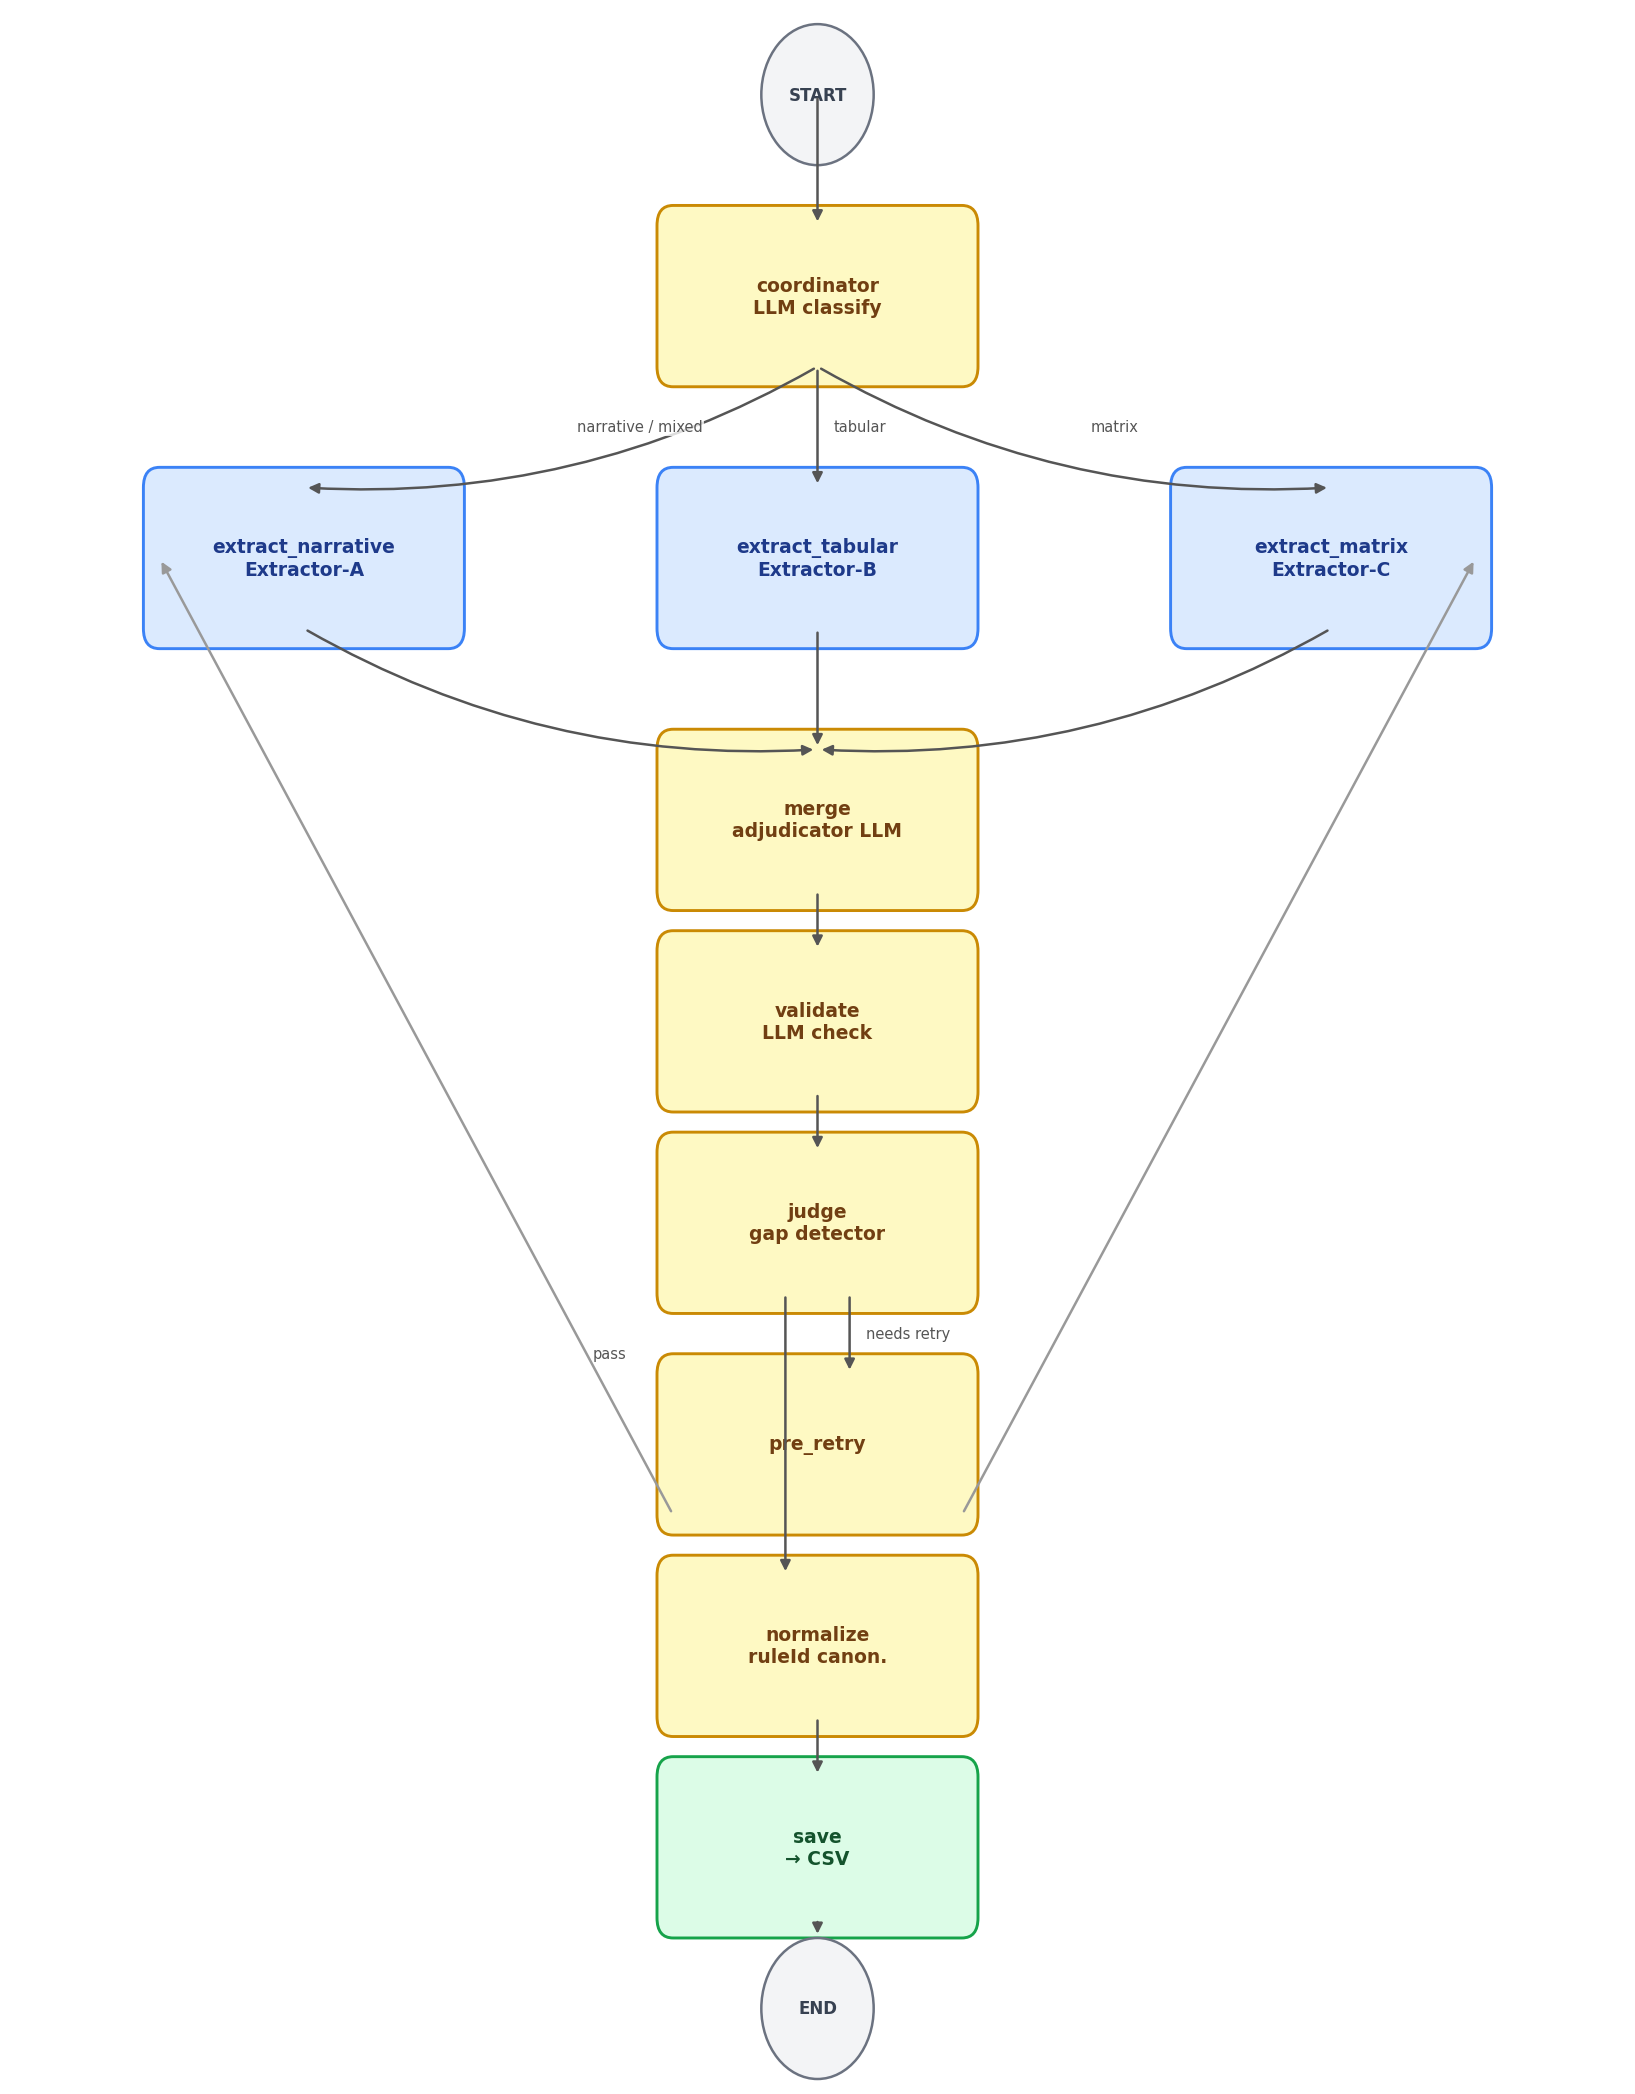
\includegraphics[width=0.60\textwidth]{pipeline_full.png}
    \caption{Pipeline computation graph implemented with LangGraph. Nodes represent
             processing stages; solid edges represent unconditional data flow, dashed
             edges represent conditional routing after the Judge.}
    \label{fig:pipeline_full}
\end{figure}

\subsection{Error Resilience Strategy}
\label{sec:error_resilience}

Every LLM-calling node is wrapped in an exponential-backoff retry loop (up to
\texttt{MAX\_RETRIES} attempts). If a node exhausts its retries, the pipeline
continues with an empty rule list where appropriate, and the Consensus Merger
includes a fallback that re-invokes the extractor if its input is empty. The JSON
parser (\texttt{parse\_rules}) used throughout handles Markdown fences, truncated
arrays, and malformed objects, so that even imperfect LLM output can be salvaged.

% ==============================================================================
\section{Ablation Study and Results}
\label{sec:ablation}

To quantify the contribution of each pipeline stage, an ablation study was
conducted using the iMAKS dataset and the evaluation protocol described in
Section~\ref{sec:evaluation}. The study systematically disables or simplifies one
component at a time and measures the resulting change in extraction quality. All
experiments were run with random seed~42 and the same model assignments
(Table~\ref{tab:node_roles}).

\subsection{Ablation Configurations}
\label{sec:ablation_configs}

Five ablation conditions, plus the full pipeline baseline and a deterministic
regex parser, were tested. Table~\ref{tab:ablation_configs} summarises each
condition, the modified component, and the scientific question it addresses.

\begin{table}[htbp]
\centering
\caption{Ablation conditions and the scientific questions they address.}
\label{tab:ablation_configs}
\resizebox{\textwidth}{!}{%
\begin{tabular}{@{}llp{8cm}@{}}
\toprule
\textbf{Output file} & \textbf{Modified component} & \textbf{Question addressed} \\
\midrule
\texttt{ext\_multi\_agent\_langgraph} (full)
  & All nodes present
  & Reference baseline; complete pipeline. \\
\texttt{abl\_noJudge}
  & QualityGapEvaluator and retry loop removed
  & How much does the iterative judge loop improve recall? \\
\texttt{abl\_noValidator}
  & Validator replaced by deterministic filter only
  & How many false positives and false negatives does the Validator catch? \\
\texttt{abl\_noAdj}
  & Adjudicator replaced by deterministic-only merge (Branch~D keeps all
    conflicting candidates)
  & Does LLM conflict resolution outperform purely deterministic deduplication? \\
\texttt{abl\_noCM}
  & LLM Coordinator replaced by keyword/regex classifier
  & Is a learned document-type classifier necessary, or can simple heuristics
    suffice? \\
\texttt{baseline\_b0} (deterministic)
  & Deterministic regex parser with hard-coded knowledge of the factory nodes
  & How well can a hand-crafted parser perform on this structured dataset? \\
\bottomrule
\end{tabular}%
}
\end{table}

All components not listed as modified---including the extractor prompts, the
deterministic post-filter, and the Normalizer---are identical across every
LLM-based condition, ensuring a fair comparison.

\subsection{Implementation of Ablation Variants}
\label{sec:ablation_impl}

Each ablation variant is built as an independent \texttt{StateGraph} by the
function \texttt{build\_graph(ablation)}. This avoids runtime branching complexity
and ensures every condition is a clean, auditable pipeline definition.

\paragraph{No LLM Coordinator (\texttt{abl\_noCM}).}
The \texttt{Coordinator} node is replaced by a regex-based classifier.
Document types are inferred by matching patterns: \texttt{CRIT\_LO|WARN\_LO|WARN\_HI|CRIT\_HI}
triggers \texttt{tabular}, role-vs-zone matrices trigger \texttt{matrix},
maintenance-specific keywords trigger \texttt{mixed}, and everything else defaults
to \texttt{narrative}.

\paragraph{No LLM Adjudicator (\texttt{abl\_noAdj}).}
The \texttt{ConsensusMerger} node is replaced by a deterministic-only variant.
Branches~A through~C remain identical. However, for Branch~D (genuine conflicts),
all candidates are kept without LLM resolution.

\paragraph{No Validator (\texttt{abl\_noValidator}).}
The \texttt{Validator} node is replaced by a passthrough that applies only the
deterministic post-filter. The LLM-based grounding check and false-negative
recovery are completely omitted.

\paragraph{No Judge (\texttt{abl\_noJudge}).}
The \texttt{QualityGapEvaluator} node and the associated retry loop are removed.
The graph connects the Validator directly to the Normalizer, eliminating all
re-extraction cycles.

\paragraph{Deterministic Baseline (\texttt{baseline\_b0}).}
A hand-crafted regex parser with embedded knowledge of the factory's four stations
and their sensors. It processes the four SOP document types with dedicated parsing
functions, with no LLM calls. Its output serves as a lower-bound reference for what
domain knowledge alone can achieve.

\subsection{Results}
\label{sec:ablation_results}

Table~\ref{tab:ablation_table} presents the primary metric,
F1\textsubscript{content}, along with precision, recall, and the number of
extracted rules, for each condition. Results are sorted by
F1\textsubscript{content} in descending order. Selected single-agent LLM baselines
from the grid search are included to contextualise the multi-agent pipeline's gain.

\begin{table}[htbp]
\centering
\caption{Ablation results (content metric with match counts). The ground truth
         contains 86 rules. TP, FP, FN are derived from the Hungarian assignment
         at a CA threshold of~0.6.}
\label{tab:ablation_table}
\resizebox{\textwidth}{!}{%
\begin{tabular}{@{}lccccccc@{}}
\toprule
\textbf{Configuration}
  & \textbf{F1\textsubscript{c}}
  & \textbf{P\textsubscript{c}}
  & \textbf{R\textsubscript{c}}
  & \textbf{TP\textsubscript{c}}
  & \textbf{FP\textsubscript{c}}
  & \textbf{FN\textsubscript{c}}
  & \textbf{\#Pred} \\
\midrule
\multicolumn{8}{c}{\textit{Multi-Agent Pipeline Ablations}} \\
\midrule
\texttt{ext\_multi\_agent} (full)
  & \textbf{0.823} & 0.903 & 0.756 & 65 &  7 & 21 & 72 \\
\texttt{abl\_noJudge}
  & 0.795 & 0.923 & 0.698 & 60 &  5 & 26 & 65 \\
\texttt{abl\_noValidator}
  & 0.776 & 0.934 & 0.663 & 57 &  4 & 29 & 61 \\
\texttt{abl\_noCM}
  & 0.761 & 0.855 & 0.686 & 59 & 10 & 27 & 69 \\
\texttt{abl\_noAdj}
  & 0.703 & 0.864 & 0.593 & 51 &  8 & 35 & 59 \\
\texttt{baseline\_b0} (deterministic)
  & 0.634 & 0.804 & 0.523 & 45 & 11 & 41 & 56 \\
\midrule
\multicolumn{8}{c}{\textit{Best Single-Agent LLM Baselines (grid search)}} \\
\midrule
\texttt{gpt-oss-20b} (few-shot)
  & 0.728 & 0.846 & 0.640 & 55 & 10 & 31 & 65 \\
\texttt{ministral-3-8b} (few-shot)
  & 0.727 & 0.759 & 0.698 & 60 & 19 & 26 & 79 \\
\texttt{ministral-3-14b} (few-shot)
  & 0.726 & 0.744 & 0.709 & 61 & 21 & 25 & 82 \\
\bottomrule
\end{tabular}%
}
\end{table}

\subsection{Interpretation}
\label{sec:ablation_interpretation}

\textbf{Full pipeline superiority.}
The complete multi-agent pipeline achieves the highest
F1\textsubscript{content}~(0.823), outperforming the best single-agent few-shot
baseline~(0.728) by 0.095 points (approximately 13\% relative improvement).
Its recall~(0.756) is substantially higher than any single-agent approach, while
maintaining high precision~(0.903). The 65 true positive matches represent 75.6\%
of the 86 ground-truth rules.

\textbf{Impact of the Quality Gap Evaluator.}
Removing the judge loop (\texttt{abl\_noJudge}) drops
F1\textsubscript{content} to 0.795, a loss of 0.028 points. Precision increases
slightly~(0.923), but recall falls from 0.756 to 0.698, confirming that the
iterative refinement primarily boosts recall by recovering rules missed in a single
extraction pass.

\textbf{Importance of the Validator.}
Without the Validator (\texttt{abl\_noValidator}),
F1\textsubscript{content} decreases to 0.776. Although precision remains high
(0.934) due to the deterministic post-filter, recall drops to 0.663, indicating
that the Validator recovers a non-trivial number of false negatives that the judge
alone cannot catch.

\textbf{Coordinator classification matters.}
Replacing the LLM-based document-type classifier with keyword heuristics
(\texttt{abl\_noCM}) reduces F1\textsubscript{content} to 0.761. Recall~(0.686)
is close to the full pipeline's, but precision falls to 0.855, suggesting that
misclassifications cause the wrong extractor prompt to be applied, introducing
noise.

\textbf{LLM adjudication vs.\ deterministic merge.}
Using only deterministic deduplication without the LLM adjudicator
(\texttt{abl\_noAdj}) yields an F1\textsubscript{content} of 0.703, the weakest
among the LLM-based ablations. Both precision~(0.864) and recall~(0.593) drop
substantially, indicating that the adjudicator improves rule coherence by resolving
genuine conflicts and preventing the same physical constraint from being represented
by multiple slightly different rules.

\textbf{Deterministic baseline.}
The hand-crafted regex parser (\texttt{baseline\_b0}) achieves a perfect strict
precision of 1.0 precisely because it relies on rigid patterns and a fixed set of
known stations and sensors. However, this brittleness restricts it to capturing
only 56~rules, resulting in F1\textsubscript{content}~=~0.634 driven by high
content precision~(0.804) but severely limited recall~(0.523). Any change to the
SOP layout or node inventory would require manual re-engineering, underscoring the
flexibility advantage of the LLM-based pipeline.

\textbf{Overall conclusion.}
The ablation study confirms that every component of the pipeline contributes
positively. The iterative judge loop boosts recall, the Validator cleans false
positives and recovers omissions, the Adjudicator improves rule coherence, and the
LLM Coordinator ensures that each document is processed with the most appropriate
extraction prompt. Together, they enable the collaborative multi-agent pipeline to
surpass not only individual LLM agents but also a carefully tuned deterministic
parser.

% ==============================================================================
\section{Knowledge Graph Construction and Integration}
\label{sec:neo4j}

Once the multi-agent pipeline produces its best extraction run, the extracted rules
are loaded into a Neo4j graph database where they are overlaid on a hand-crafted
ground-truth graph (the ABox) that encodes the factory's physical structure and
operational history.
The integration proceeds in four sequential steps, implemented in the
\texttt{layer\_4/} module: ABox loading (\texttt{step4}), extracted rule overlay
(\texttt{step5}), typed triplet enrichment (\texttt{step7}), and a graph-level
coverage evaluation (\texttt{step6}).

\subsection{ABox Design and Loading}
\label{sec:abox}

The ABox is the hand-crafted ground-truth graph that captures the complete
structure of the iMAKS industrial facility.
It is stored as two CSV files (\texttt{nodes.csv}, \texttt{edges.csv}) in
\texttt{data/dataset/kg\_seed/} and loaded into Neo4j by
\texttt{step4\_neo4j\_loader.py}.

\subsubsection{Node Types}

The ABox contains 115 nodes of eight semantic types:

\begin{itemize}
    \item \textbf{System (1)} --- the top-level \texttt{iMAKS} node representing
          the entire food-packaging facility.
    \item \textbf{Zone (7)} --- physical areas of the facility: Production Area,
          Server Room, General Warehouse, Main Entrance, Chemical Storage,
          R\&D Lab, and Cafeteria. Each zone acts as a security and operational
          boundary.
    \item \textbf{Component (9)} --- production stations and auxiliary rooms
          (e.g.\ \texttt{ST01\_FILLING}, \texttt{ST02\_SEALING},
          \texttt{SRV01\_SERVERROOM}), each associated with a zone and a station
          type.
    \item \textbf{Sensor (22)} --- physical measurement devices attached to
          components (e.g.\ \texttt{ST01\_FILLING\_TMP},
          \texttt{ST02\_SEALING\_CUR}). Each sensor node carries its nominal value,
          warning bounds (\texttt{warnLo}, \texttt{warnHi}), critical bounds
          (\texttt{critLo}, \texttt{critHi}), unit, and sensor type
          (TMP, PRS, FLW, CUR, SPD, VIB, TEN, CNT, HUM).
    \item \textbf{AnomalyEvent (14)} --- recorded fault events from five days of
          simulated operations (e.g.\ \texttt{GT-0009}: a correlated speed anomaly
          at the packaging station caused by a current drift at the sealing station
          90 minutes upstream).
    \item \textbf{Maintenance (8)} --- scheduled or reactive maintenance procedures,
          each keyed by a \texttt{ruleId} (MAINT-01 through MAINT-08) and a
          priority (CRITICAL, HIGH, MEDIUM).
    \item \textbf{Person (44)} --- factory personnel with assigned roles (operator,
          engineer, manager, chemist, etc.) and shift schedules.
    \item \textbf{SafetyEvent (10)} --- recorded safety incidents linked to zones
          and personnel.
\end{itemize}

\subsubsection{Edge Types}

The ABox contains 341 edges of ten semantic types:

\begin{itemize}
    \item \texttt{contains} (16) --- Zone or Component $\rightarrow$ Component or
          Sensor; encodes physical containment.
    \item \texttt{part\_of} (9) --- Component $\rightarrow$ System or Zone;
          inverse structural membership.
    \item \texttt{monitors} (44) --- Component $\rightarrow$ Sensor (bidirectional
          pair); a station monitors its attached sensors.
    \item \texttt{triggers} (22) --- Sensor $\rightarrow$ AnomalyEvent or
          Maintenance; a sensor reading outside its bounds triggers the event.
    \item \texttt{resolves} (8) --- Maintenance $\rightarrow$ Sensor; the
          maintenance action resolves the root-cause sensor anomaly.
    \item \texttt{feeds\_into} (3) --- Component $\rightarrow$ Component;
          material flow in the production line.
    \item \texttt{correlates\_with} (1) --- Sensor $\rightarrow$ Sensor with
          \texttt{ruleRef} property; the key cross-station dependency that underlies
          the GT-0009 anomaly (ST02\_SEALING\_CUR correlates with
          ST04\_PACKAGING\_SPD with a 90-minute lag).
    \item \texttt{authorized\_for} (218) --- Person $\rightarrow$ Zone;
          encodes access rights for each personnel--zone pair.
    \item \texttt{detected\_in} (10) --- SafetyEvent $\rightarrow$ Zone; records
          where each safety incident was observed.
    \item \texttt{involves} (10) --- SafetyEvent $\rightarrow$ Person.
\end{itemize}

\subsubsection{Loading Procedure}

The loader wipes the graph before each run (unless \texttt{--no-clear} is passed),
creates a uniqueness constraint on \texttt{nodeId}, then writes nodes and edges via
Cypher \texttt{MERGE} statements. Each node receives both the generic \texttt{:Node}
label (for label-agnostic queries) and its semantic label (e.g.\ \texttt{:Sensor}).
After loading, a summary query confirms the correct node and edge counts.

\subsection{Extracted Rule Overlay}
\label{sec:rule_overlay}

\texttt{step5\_neo4j\_rules.py} selects the extraction run with the highest
F1\textsubscript{content} score from \texttt{evaluation\_summary.csv}
(auto-selection; a specific run file can also be provided via \texttt{--run-file})
and loads each extracted rule as a \texttt{:ExtractedRule} node in Neo4j.

\subsubsection{UID Scheme}

Each \texttt{:ExtractedRule} node is assigned a globally unique identifier:

\begin{center}
\texttt{uid = <run\_file>::<ruleId>::<row\_index>}
\end{center}

This compound key ensures uniqueness even if two extraction runs produce rules with
the same \texttt{ruleId}, and it allows step7 to reliably look up the correct node
when building the typed triplet structure.

\subsubsection{Wiring to the ABox}

After creating the \texttt{:ExtractedRule} node, the loader attempts two
connections into the ABox:

\begin{itemize}
    \item \texttt{(r:ExtractedRule)-[:COVERS]->(s:Sensor)} --- matches on the
          \texttt{sensor} field of the extracted rule against the \texttt{name}
          property of \texttt{:Sensor} nodes. This is the primary coverage link
          used by the phase-2 evaluation.
    \item \texttt{(r:ExtractedRule)-[:APPLIES\_TO]->(c:Component)} --- matches on
          the \texttt{station} field against \texttt{:Component} names.
\end{itemize}

For the best run (\texttt{ext\_multi\_agent\_langgraph.csv}, 72 rules), the loader
created 49 \texttt{:COVERS} edges and 50 \texttt{:APPLIES\_TO} edges, leaving 23
rules without a sensor match and 22 without a station match. Unmatched rules are
typically access rules (which reference zones rather than sensors) or maintenance
rules where the LLM assigned a non-standard sensor name.

\subsection{Typed Triplet Enrichment}
\label{sec:triplets}

\texttt{step7\_rule\_to\_triplets.py} converts the flat \texttt{:ExtractedRule}
nodes into a richer, semantically typed sub-graph. The enrichment is class-aware:
different rule classes produce different node and edge types.

\subsubsection{ThresholdRule Enrichment}

For each \texttt{ThresholdRule} that carries at least one numeric threshold value,
a \texttt{:ThresholdSpec} node is created with properties
\texttt{critHi}, \texttt{warnHi}, \texttt{warnLo}, \texttt{critLo}, and
\texttt{unit}. Two typed edges connect it to the rest of the graph:

\begin{itemize}
    \item \texttt{(r:ExtractedRule)-[:HAS\_SPEC]->(ts:ThresholdSpec)} --- links the
          rule to its numeric specification.
    \item \texttt{(ts:ThresholdSpec)-[:GOVERNS \{critHi, warnHi, \ldots\}]->(s:Sensor)}
          --- carries the threshold values directly on the relationship, enabling
          one-hop Cypher queries to check whether a live sensor reading violates any
          extracted threshold (e.g.\ \texttt{MATCH (ts)-[g:GOVERNS]->(s) WHERE
          s.name = \$sensorId RETURN g.critHi}).
\end{itemize}

From the 72 extracted rules, 46 \texttt{:ThresholdSpec} nodes, 46
\texttt{:HAS\_SPEC} edges, and 46 \texttt{:GOVERNS} edges were created.

\subsubsection{OperationalRule and MaintenanceRule Enrichment}

For each \texttt{OperationalRule} or \texttt{MaintenanceRule} node:

\begin{itemize}
    \item \texttt{(s:Sensor)-[:TRIGGERS\_RULE]->(r:ExtractedRule)} --- reverse edge
          from the sensor to the rule it activates; 3 edges created.
    \item \texttt{(r:ExtractedRule)-[:REQUIRES\_ACTION]->(a:Action)} --- an
          \texttt{:Action} node is created holding the \texttt{text} (prescribed
          response) and \texttt{severity} properties; 3 nodes and 3 edges created.
\end{itemize}

\subsubsection{AccessRule Enrichment}

Access rules are linked to the zone they restrict via a station-to-zone lookup table
mapping codes such as \texttt{CHM01\_CHEMICALSTORAGE} to \texttt{Chemical Storage}:

\begin{itemize}
    \item \texttt{(r:ExtractedRule)-[:RESTRICTS\_ACCESS]->(z:Zone)} ---
          1 edge created.
\end{itemize}

\subsubsection{Cross-Station Dependency Detection}

A heuristic cross-station dependency detector scans each rule's \texttt{condition}
text for station keywords (e.g.\ \texttt{ST02}, \texttt{SEALING}) that differ from
the rule's own station. If a foreign station is mentioned, a
\texttt{(src:ExtractedRule)-[:DEPENDS\_ON]->(tgt:ExtractedRule)} edge is created to
every rule from that foreign station. This heuristic encodes the GT-0009 causal
pattern (a packaging rule that mentions the sealing station as its upstream cause)
without requiring explicit LLM annotation of dependencies.
No such edges were created for the current best run, confirming that the
multi-agent pipeline did not capture the cross-station causal reasoning required
by GT-0009 (see Section~\ref{sec:phase2_results}).

\subsection{Phase-2 Graph Coverage Evaluation}
\label{sec:phase2_results}

The phase-2 evaluation (\texttt{step6\_phase2\_evaluation.py}) tests whether the
extracted rules, as loaded into Neo4j, provide sufficient coverage of the real
operational events recorded in the ABox.
Unlike the F1\textsubscript{content} metric (which compares rules in isolation),
this evaluation traverses the graph: it asks whether the \emph{connected} extraction
layer adequately ``guards'' the ABox's fault and maintenance nodes.

\subsubsection{Coverage of Anomaly Events}

For each of the 14 \texttt{:AnomalyEvent} nodes in the ABox, the evaluator checks
whether at least one \texttt{:ExtractedRule} covers the sensor that triggered it:

\begin{center}
\texttt{MATCH (s:Sensor)-[:triggers]->(ae:AnomalyEvent)}\\
\texttt{OPTIONAL MATCH (r:ExtractedRule)-[:COVERS]->(s)}\\
\texttt{RETURN ae.gtId, count(r) AS coveringRules}
\end{center}

\noindent All 14/14 anomaly events are covered, including the six most common
fault types (SPIKE, DRIFT, STUCK, OUT\_OF\_RANGE, CORRELATED).

\subsubsection{Coverage of Maintenance Procedures}

For each of the 8 \texttt{:Maintenance} nodes, the evaluator traverses the
\texttt{Sensor-[:triggers]->Maintenance} path and checks whether any
\texttt{:ExtractedRule} of class \texttt{MaintenanceRule} covers the same sensor:

\begin{center}
\texttt{MATCH (s:Sensor)-[:triggers]->(m:Maintenance)}\\
\texttt{OPTIONAL MATCH (r:ExtractedRule)-[:COVERS]->(s)}\\
\texttt{WHERE r.ruleClass IN ['MaintenanceRule', ...]}
\end{center}

\noindent Only 2/8 maintenance procedures are covered, corresponding exactly to the
two \texttt{MaintenanceRule} entries extracted from SOP-003 by the multi-agent
pipeline (MAINT-02 at \texttt{ST02\_SEALING\_CUR} and MAINT-03 at
\texttt{ST03\_LABELLING\_TEN}).
The six uncovered procedures correspond to sensors for which the pipeline extracted
\texttt{ThresholdRule} or \texttt{OperationalRule} entries instead of the
operationally correct \texttt{MaintenanceRule} class.

\subsubsection{Overall Coverage and the 70\% Threshold}

Table~\ref{tab:phase2} summarises the phase-2 results.

\begin{table}[htbp]
\centering
\caption{Phase-2 graph coverage evaluation results for the best extraction run
         (\texttt{ext\_multi\_agent\_langgraph}, F1\textsubscript{content}~=~0.823).}
\label{tab:phase2}
\begin{tabular}{@{}lrrl@{}}
\toprule
\textbf{Event type} & \textbf{Covered} & \textbf{Total} & \textbf{Status} \\
\midrule
AnomalyEvents & 14 & 14 & \textbf{100\%} \\
Maintenance   &  2 &  8 & 25\% \\
\midrule
\textbf{Overall} & \textbf{16} & \textbf{22} & \textbf{72.7\%} $\geq$ 70\% \checkmark \\
\bottomrule
\end{tabular}
\end{table}

The 72.7\% overall coverage exceeds the 70\% design threshold specified in the
iMAKS dataset guide, confirming that the pipeline's extracted rules are
operationally sufficient for the anomaly-detection use case, even though the
maintenance coverage gap signals a remaining extraction weakness in
domain-specific procedure identification.

\subsubsection{GT-0009: Multi-Source Causal Fusion Test}
\label{sec:gt0009}

GT-0009 is the hardest test case in the benchmark: a speed anomaly at
\texttt{ST04\_PACKAGING} is caused by a current drift at \texttt{ST02\_SEALING}
with a 90-minute lag, encoded in the ABox as a
\texttt{correlates\_with \{ruleRef: RULE-ST02-04\}} edge between the two sensors.
Passing the GT-0009 test requires an extracted rule that (1) covers sensor
\texttt{ST04\_PACKAGING\_SPD} \emph{and} (2) references the sealing station or
ST02 as the upstream cause in its \texttt{condition} text.

The pipeline \emph{passes condition~(1)}: the extracted rule set contains a rule
covering \texttt{ST04\_PACKAGING\_SPD}.
It \emph{fails condition~(2)}: no extracted rule mentions ST02 or the sealing
station as a causal origin in its condition text.
The cross-station dependency therefore remains implicit in the ABox's
\texttt{correlates\_with} edge but was not surfaced by any agent.
This finding confirms that multi-source causal fusion is a systematic gap for
current single-pass LLM extractors and motivates future work on graph-informed
prompting strategies that explicitly provide the ABox's correlation edges to the
extraction agent.

\subsection{Extraction Error Analysis in the KG Context}
\label{sec:error_analysis}

Loading the extracted rules into Neo4j exposes a class of failure modes that are
invisible when evaluating rules as isolated text strings.
Two systematic errors are observable by inspecting the \texttt{:GOVERNS} edges and
their numeric properties.

\subsubsection{Temporal Drift Threshold Confusion}

Several \texttt{:GOVERNS} edges carry threshold values that are semantically
inconsistent with the sensor's nominal operating range stored in the ABox.
For example:

\begin{itemize}
    \item \texttt{ST02\_SEALING\_CUR} (nominal 12.4\,A, \texttt{critHi}~=~15.0\,A
          in the ABox) has a \texttt{GOVERNS} edge with
          \texttt{\{unit: A, critHi: 1.0\}}.
          The value 1.0\,A derives from the SOP-003 maintenance rule
          ``CUR DRIFT $>$1.0\,A for 30+ min'' --- a \emph{drift magnitude},
          not a static alarm limit.
          The LLM extracted the drift threshold as a \texttt{critHi} value and
          assigned it to a \texttt{ThresholdRule}, causing a 15$\times$ underestimate
          of the true critical current.
    \item \texttt{ST04\_PACKAGING\_VIB} (\texttt{critHi}~=~0.35\,mm/s in the ABox)
          has a \texttt{GOVERNS} edge with \texttt{\{unit: mm/s, critHi: 0.05\}}.
          The value 0.05\,mm/s originates from the maintenance condition
          ``VIB DRIFT $>$0.05\,mm/s over 60\,min'' and was similarly
          misclassified as a static critical threshold.
\end{itemize}

In both cases the LLM failed to distinguish between a \emph{static bound}
(absolute sensor limit) and a \emph{temporal drift constraint}
(rate of change over a time window). A static bound should be extracted as a
\texttt{ThresholdRule} with the absolute value; a temporal drift constraint should
be extracted as a \texttt{MaintenanceRule} with the drift rate in the
\texttt{condition} field.

This confusion category is directly responsible for a portion of the 6/8
maintenance coverage gap: several maintenance rules were extracted as
threshold rules, leading to their type mismatch in the phase-2 evaluation.

\subsubsection{Unit Dimension Mismatch}

A secondary error is visible in the \texttt{ST03\_LABELLING\_TEN} sensor, where one
\texttt{:GOVERNS} edge carries \texttt{\{unit: samples, critLo: 10.0\}}.
The sensor's native unit is Newton (N), but the LLM correctly identified the STUCK
condition (``$>$10 consecutive samples without change'') and expressed it in the
operationally meaningful unit of \emph{samples}.
While semantically valid, this introduces a unit-dimension mismatch relative to the
ABox sensor properties, which would cause a type error in any downstream reasoner
that directly compares \texttt{GOVERNS.unit} against \texttt{Sensor.unit}.
This class of error motivates unit normalisation as a post-processing step in future
pipeline versions.

% ==============================================================================
\appendix
\section{Complete Evaluation Results}
\label{app:full_results}

This appendix lists the complete evaluation results, grouped by model (and by
special system or ablation). Within each group, experiments are sorted by
F1\textsubscript{content} in descending order. Each row reports the total number
of extracted rules (\#Ext), strict identifier match metrics (S\nobreakdash-F1,
S\nobreakdash-P, S\nobreakdash-R, S\nobreakdash-TP, S\nobreakdash-FP,
S\nobreakdash-FN), and content-based metrics (C\nobreakdash-F1,
C\nobreakdash-P, C\nobreakdash-R, C\nobreakdash-TP, C\nobreakdash-FP,
C\nobreakdash-FN). Content match counts are derived from the Hungarian assignment
with a similarity threshold of~0.6.

\subsection*{Multi-Agent System and Ablations}
\begin{table}[H]
\centering
\caption{Results for the multi-agent system, ablations, and the deterministic
         baseline.}
\label{tab:multi_agent_abl}
\resizebox{\textwidth}{!}{%
\begin{tabular}{@{}lccccccccccccc@{}}
\toprule
\textbf{Configuration}
  & \textbf{\#Ext}
  & \textbf{S-F1} & \textbf{S-P} & \textbf{S-R}
  & \textbf{S-TP} & \textbf{S-FP} & \textbf{S-FN}
  & \textbf{C-F1} & \textbf{C-P} & \textbf{C-R}
  & \textbf{C-TP} & \textbf{C-FP} & \textbf{C-FN} \\
\midrule
\texttt{ext\_multi\_agent\_langgraph}
  & 72 & 0.558 & 0.632 & 0.500 & 43 & 25 & 43
  & 0.823 & 0.903 & 0.756 & 65 &  7 & 21 \\
\texttt{abl\_noJudge\_s42\_run1}
  & 65 & 0.531 & 0.639 & 0.453 & 39 & 22 & 47
  & 0.795 & 0.923 & 0.698 & 60 &  5 & 26 \\
\texttt{abl\_noValidator\_s42\_run1}
  & 61 & 0.583 & 0.724 & 0.488 & 42 & 16 & 44
  & 0.776 & 0.934 & 0.663 & 57 &  4 & 29 \\
\texttt{abl\_noCM\_s42\_run1}
  & 69 & 0.632 & 0.710 & 0.570 & 49 & 20 & 37
  & 0.761 & 0.855 & 0.686 & 59 & 10 & 27 \\
\texttt{abl\_noAdj\_s42\_run1}
  & 59 & 0.556 & 0.690 & 0.465 & 40 & 18 & 46
  & 0.703 & 0.864 & 0.593 & 51 &  8 & 35 \\
\texttt{baseline\_b0}
  & 56 & 0.789 & 1.000 & 0.651 & 56 &  0 & 30
  & 0.634 & 0.804 & 0.523 & 45 & 11 & 41 \\
\bottomrule
\end{tabular}%
}
\end{table}

\subsection*{GPT-OSS-20B}
\begin{table}[H]
\centering
\caption{Results for the \texttt{gpt-oss-20b} model.}
\label{tab:gpt_oss_20b}
\resizebox{\textwidth}{!}{%
\begin{tabular}{@{}lccccccccccccc@{}}
\toprule
\textbf{Configuration}
  & \textbf{\#Ext}
  & \textbf{S-F1} & \textbf{S-P} & \textbf{S-R}
  & \textbf{S-TP} & \textbf{S-FP} & \textbf{S-FN}
  & \textbf{C-F1} & \textbf{C-P} & \textbf{C-R}
  & \textbf{C-TP} & \textbf{C-FP} & \textbf{C-FN} \\
\midrule
\texttt{ext\_gpt-oss-20b\_few\_shot\_static\_s42}
  & 65 & 0.411 & 0.477 & 0.360 & 31 & 34 & 55
  & 0.728 & 0.846 & 0.640 & 55 & 10 & 31 \\
\texttt{ext\_gpt-oss-20b\_reflexion\_s42}
  & 65 & 0.397 & 0.462 & 0.349 & 30 & 35 & 56
  & 0.662 & 0.769 & 0.581 & 50 & 15 & 36 \\
\texttt{ext\_gpt-oss-20b\_reflexion\_guided\_s42}
  & 89 & 0.380 & 0.403 & 0.360 & 31 & 46 & 55
  & 0.617 & 0.607 & 0.628 & 54 & 35 & 32 \\
\texttt{ext\_gpt-oss-20b\_react\_abox\_s42}
  & 64 & 0.400 & 0.469 & 0.349 & 30 & 34 & 56
  & 0.613 & 0.719 & 0.535 & 46 & 18 & 40 \\
\texttt{ext\_gpt-oss-20b\_graph\_informed\_s42}
  & 63 & 0.416 & 0.492 & 0.360 & 31 & 32 & 55
  & 0.510 & 0.603 & 0.442 & 38 & 25 & 48 \\
\texttt{ext\_gpt-oss-20b\_pre\_act\_s42}
  & 78 & 0.341 & 0.359 & 0.326 & 28 & 50 & 58
  & 0.500 & 0.526 & 0.477 & 41 & 37 & 45 \\
\texttt{ext\_gpt-oss-20b\_naive\_s42}
  & 66 & 0.422 & 0.508 & 0.360 & 31 & 30 & 55
  & 0.461 & 0.530 & 0.407 & 35 & 31 & 51 \\
\texttt{ext\_gpt-oss-20b\_cot\_basic\_s42}
  & 66 & 0.355 & 0.409 & 0.314 & 27 & 39 & 59
  & 0.447 & 0.515 & 0.395 & 34 & 32 & 52 \\
\texttt{ext\_gpt-oss-20b\_self\_consistency\_s42}
  & 63 & 0.349 & 0.413 & 0.302 & 26 & 37 & 60
  & 0.443 & 0.524 & 0.384 & 33 & 30 & 53 \\
\texttt{ext\_gpt-oss-20b\_cot\_structured\_s42}
  & 88 & 0.356 & 0.352 & 0.360 & 31 & 57 & 55
  & 0.149 & 0.148 & 0.151 & 13 & 75 & 73 \\
\bottomrule
\end{tabular}%
}
\end{table}

\subsection*{Gemma3-12B}
\begin{table}[H]
\centering
\caption{Results for the \texttt{gemma3:12b} model.}
\label{tab:gemma3_12b}
\resizebox{\textwidth}{!}{%
\begin{tabular}{@{}lccccccccccccc@{}}
\toprule
\textbf{Configuration}
  & \textbf{\#Ext}
  & \textbf{S-F1} & \textbf{S-P} & \textbf{S-R}
  & \textbf{S-TP} & \textbf{S-FP} & \textbf{S-FN}
  & \textbf{C-F1} & \textbf{C-P} & \textbf{C-R}
  & \textbf{C-TP} & \textbf{C-FP} & \textbf{C-FN} \\
\midrule
\texttt{ext\_gemma3-12b\_graph\_informed\_s42}
  & 65 & 0.403 & 0.476 & 0.349 & 30 & 33 & 56
  & 0.649 & 0.754 & 0.570 & 49 & 16 & 37 \\
\texttt{ext\_gemma3-12b\_react\_abox\_s42}
  & 66 & 0.465 & 0.698 & 0.349 & 30 & 13 & 56
  & 0.605 & 0.697 & 0.535 & 46 & 20 & 40 \\
\texttt{ext\_gemma3-12b\_reflexion\_s42}
  & 77 & 0.373 & 0.400 & 0.349 & 30 & 45 & 56
  & 0.601 & 0.636 & 0.570 & 49 & 28 & 37 \\
\texttt{ext\_gemma3-12b\_few\_shot\_static\_s42}
  & 65 & 0.702 & 0.815 & 0.616 & 53 & 12 & 33
  & 0.583 & 0.677 & 0.512 & 44 & 21 & 42 \\
\texttt{ext\_gemma3-12b\_reflexion\_guided\_s42}
  & 80 & 0.370 & 0.395 & 0.349 & 30 & 46 & 56
  & 0.566 & 0.588 & 0.547 & 47 & 33 & 39 \\
\texttt{ext\_gemma3-12b\_naive\_s42}
  & 65 & 0.488 & 0.756 & 0.360 & 31 & 10 & 55
  & 0.424 & 0.492 & 0.372 & 32 & 33 & 54 \\
\texttt{ext\_gemma3-12b\_pre\_act\_s42}
  & 71 & 0.397 & 0.443 & 0.360 & 31 & 39 & 55
  & 0.420 & 0.465 & 0.384 & 33 & 38 & 53 \\
\texttt{ext\_gemma3-12b\_cot\_structured\_s42}
  & 68 & 0.458 & 0.667 & 0.349 & 30 & 15 & 56
  & 0.416 & 0.471 & 0.372 & 32 & 36 & 54 \\
\texttt{ext\_gemma3-12b\_self\_consistency\_s42}
  & 65 & 0.488 & 0.756 & 0.360 & 31 & 10 & 55
  & 0.411 & 0.477 & 0.360 & 31 & 34 & 55 \\
\texttt{ext\_gemma3-12b\_cot\_basic\_s42}
  & 63 & 0.419 & 0.500 & 0.360 & 31 & 31 & 55
  & 0.376 & 0.444 & 0.326 & 28 & 35 & 58 \\
\bottomrule
\end{tabular}%
}
\end{table}

\subsection*{Ministral-3-14B}
\begin{table}[H]
\centering
\caption{Results for the \texttt{ministral-3:14b} model.}
\label{tab:ministral_14b}
\resizebox{\textwidth}{!}{%
\begin{tabular}{@{}lccccccccccccc@{}}
\toprule
\textbf{Configuration}
  & \textbf{\#Ext}
  & \textbf{S-F1} & \textbf{S-P} & \textbf{S-R}
  & \textbf{S-TP} & \textbf{S-FP} & \textbf{S-FN}
  & \textbf{C-F1} & \textbf{C-P} & \textbf{C-R}
  & \textbf{C-TP} & \textbf{C-FP} & \textbf{C-FN} \\
\midrule
\texttt{ext\_ministral-3-14b\_few\_shot\_static\_s42}
  & 82 & 0.527 & 0.543 & 0.512 & 44 & 37 & 42
  & 0.726 & 0.744 & 0.709 & 61 & 21 & 25 \\
\texttt{ext\_ministral-3-14b\_reflexion\_s42}
  & 70 & 0.333 & 0.371 & 0.302 & 26 & 44 & 60
  & 0.615 & 0.686 & 0.558 & 48 & 22 & 38 \\
\texttt{ext\_ministral-3-14b\_graph\_informed\_s42}
  & 80 & 0.448 & 0.468 & 0.430 & 37 & 42 & 49
  & 0.614 & 0.637 & 0.593 & 51 & 29 & 35 \\
\texttt{ext\_ministral-3-14b\_react\_abox\_s42}
  & 78 & 0.380 & 0.403 & 0.360 & 31 & 46 & 55
  & 0.585 & 0.615 & 0.558 & 48 & 30 & 38 \\
\texttt{ext\_ministral-3-14b\_reflexion\_guided\_s42}
  & 108 & 0.337 & 0.337 & 0.337 & 29 & 57 & 57
  & 0.433 & 0.389 & 0.488 & 42 & 66 & 44 \\
\texttt{ext\_ministral-3-14b\_cot\_basic\_s42}
  & 76 & 0.383 & 0.408 & 0.360 & 31 & 45 & 55
  & 0.469 & 0.500 & 0.442 & 38 & 38 & 48 \\
\texttt{ext\_ministral-3-14b\_self\_consistency\_s42}
  & 73 & 0.456 & 0.620 & 0.360 & 31 & 19 & 55
  & 0.415 & 0.452 & 0.384 & 33 & 40 & 53 \\
\texttt{ext\_ministral-3-14b\_cot\_structured\_s42}
  & 85 & 0.408 & 0.492 & 0.349 & 30 & 31 & 56
  & 0.409 & 0.412 & 0.407 & 35 & 50 & 51 \\
\texttt{ext\_ministral-3-14b\_naive\_s42}
  & 82 & 0.428 & 0.525 & 0.360 & 31 & 28 & 55
  & 0.393 & 0.402 & 0.384 & 33 & 49 & 53 \\
\texttt{ext\_ministral-3-14b\_pre\_act\_s42}
  & 81 & 0.373 & 0.388 & 0.360 & 31 & 49 & 55
  & 0.371 & 0.383 & 0.360 & 31 & 50 & 55 \\
\bottomrule
\end{tabular}%
}
\end{table}

\subsection*{Ministral-3-8B}
\begin{table}[H]
\centering
\caption{Results for the \texttt{ministral-3:8b} model.}
\label{tab:ministral_8b}
\resizebox{\textwidth}{!}{%
\begin{tabular}{@{}lccccccccccccc@{}}
\toprule
\textbf{Configuration}
  & \textbf{\#Ext}
  & \textbf{S-F1} & \textbf{S-P} & \textbf{S-R}
  & \textbf{S-TP} & \textbf{S-FP} & \textbf{S-FN}
  & \textbf{C-F1} & \textbf{C-P} & \textbf{C-R}
  & \textbf{C-TP} & \textbf{C-FP} & \textbf{C-FN} \\
\midrule
\texttt{ext\_ministral-3-8b\_few\_shot\_static\_s42}
  & 79 & 0.606 & 0.633 & 0.581 & 50 & 29 & 36
  & 0.727 & 0.759 & 0.698 & 60 & 19 & 26 \\
\texttt{ext\_ministral-3-8b\_reflexion\_s42}
  & 80 & 0.431 & 0.534 & 0.360 & 31 & 27 & 55
  & 0.554 & 0.575 & 0.535 & 46 & 34 & 40 \\
\texttt{ext\_ministral-3-8b\_react\_abox\_s42}
  & 76 & 0.395 & 0.421 & 0.372 & 32 & 44 & 54
  & 0.543 & 0.579 & 0.512 & 44 & 32 & 42 \\
\texttt{ext\_ministral-3-8b\_graph\_informed\_s42}
  & 83 & 0.431 & 0.534 & 0.360 & 31 & 27 & 55
  & 0.533 & 0.542 & 0.523 & 45 & 38 & 41 \\
\texttt{ext\_ministral-3-8b\_pre\_act\_s42}
  & 78 & 0.378 & 0.397 & 0.360 & 31 & 47 & 55
  & 0.402 & 0.423 & 0.384 & 33 & 45 & 53 \\
\texttt{ext\_ministral-3-8b\_cot\_structured\_s42}
  & 93 & 0.348 & 0.337 & 0.360 & 31 & 61 & 55
  & 0.324 & 0.312 & 0.337 & 29 & 64 & 57 \\
\texttt{ext\_ministral-3-8b\_reflexion\_guided\_s42}
  & 73 & 0.425 & 0.517 & 0.360 & 31 & 29 & 55
  & 0.151 & 0.164 & 0.140 & 12 & 61 & 74 \\
\texttt{ext\_ministral-3-8b\_naive\_s42}
  & 172 & 0.241 & 0.181 & 0.360 & 31 & 140 & 55
  & 0.132 & 0.099 & 0.198 & 17 & 155 & 69 \\
\texttt{ext\_ministral-3-8b\_self\_consistency\_s42}
  & 157 & 0.255 & 0.197 & 0.360 & 31 & 126 & 55
  & 0.066 & 0.051 & 0.093 &  8 & 149 & 78 \\
\texttt{ext\_ministral-3-8b\_cot\_basic\_s42}
  & 171 & 0.242 & 0.182 & 0.360 & 31 & 139 & 55
  & 0.054 & 0.041 & 0.081 &  7 & 164 & 79 \\
\bottomrule
\end{tabular}%
}
\end{table}

\subsection*{Qwen3-4B}
\begin{table}[H]
\centering
\caption{Results for the \texttt{qwen/qwen3-4b-2507} model.}
\label{tab:qwen}
\resizebox{\textwidth}{!}{%
\begin{tabular}{@{}lccccccccccccc@{}}
\toprule
\textbf{Configuration}
  & \textbf{\#Ext}
  & \textbf{S-F1} & \textbf{S-P} & \textbf{S-R}
  & \textbf{S-TP} & \textbf{S-FP} & \textbf{S-FN}
  & \textbf{C-F1} & \textbf{C-P} & \textbf{C-R}
  & \textbf{C-TP} & \textbf{C-FP} & \textbf{C-FN} \\
\midrule
\texttt{ext\_qwen-qwen3-4b-2507\_few\_shot\_static\_s42}
  & 80 & 0.352 & 0.367 & 0.337 & 29 & 50 & 57
  & 0.699 & 0.725 & 0.674 & 58 & 22 & 28 \\
\texttt{ext\_qwen-qwen3-4b-2507\_react\_abox\_s42}
  & 78 & 0.356 & 0.377 & 0.337 & 29 & 48 & 57
  & 0.500 & 0.526 & 0.477 & 41 & 37 & 45 \\
\texttt{ext\_qwen-qwen3-4b-2507\_reflexion\_s42}
  & 81 & 0.458 & 0.475 & 0.442 & 38 & 42 & 48
  & 0.491 & 0.506 & 0.477 & 41 & 40 & 45 \\
\texttt{ext\_qwen-qwen3-4b-2507\_graph\_informed\_s42}
  & 81 & 0.458 & 0.475 & 0.442 & 38 & 42 & 48
  & 0.491 & 0.506 & 0.477 & 41 & 40 & 45 \\
\texttt{ext\_qwen-qwen3-4b-2507\_pre\_act\_s42}
  & 82 & 0.371 & 0.383 & 0.360 & 31 & 50 & 55
  & 0.476 & 0.488 & 0.465 & 40 & 42 & 46 \\
\texttt{ext\_qwen-qwen3-4b-2507\_cot\_basic\_s42}
  & 63 & 0.405 & 0.484 & 0.349 & 30 & 32 & 56
  & 0.456 & 0.540 & 0.395 & 34 & 29 & 52 \\
\texttt{ext\_qwen-qwen3-4b-2507\_reflexion\_guided\_s42}
  & 110 & 0.415 & 0.392 & 0.442 & 38 & 59 & 48
  & 0.449 & 0.400 & 0.512 & 44 & 66 & 42 \\
\texttt{ext\_qwen-qwen3-4b-2507\_self\_consistency\_s42}
  & 63 & 0.405 & 0.484 & 0.349 & 30 & 32 & 56
  & 0.443 & 0.524 & 0.384 & 33 & 30 & 53 \\
\texttt{ext\_qwen-qwen3-4b-2507\_naive\_s42}
  & 63 & 0.405 & 0.484 & 0.349 & 30 & 32 & 56
  & 0.443 & 0.524 & 0.384 & 33 & 30 & 53 \\
\texttt{ext\_qwen-qwen3-4b-2507\_cot\_structured\_s42}
  & 68 & 0.408 & 0.470 & 0.360 & 31 & 35 & 55
  & 0.403 & 0.456 & 0.360 & 31 & 37 & 55 \\
\bottomrule
\end{tabular}%
}
\end{table}

\noindent\textbf{Note:} In all tables, \textbf{S-} denotes the strict identifier
match metric and \textbf{C-} denotes the content-based metric. \textbf{\#Ext} is
the total number of extracted (predicted) rules. TP, FP, FN are the match counts
after Hungarian assignment (content) or identifier set operations (strict).

\end{document}
